\documentclass[aspectratio=169, 11pt]{beamer}

% Remover qualquer decoração de tema clássico
\usetheme{default}
\useinnertheme{rectangles}

% Remover barra de navegação superior e símbolos
\setbeamertemplate{navigation symbols}{}
\setbeamertemplate{headline}{}

% Cores modernas, flat e com ótimo contraste
\definecolor{primary}{HTML}{0D1B2A}      % Azul Escuro Profundo (Quase Preto)
\definecolor{secondary}{HTML}{415A77}    % Azul Muted/Slate
\definecolor{accent}{HTML}{E07A5F}       % Laranja Queimado Moderno
\definecolor{bglight}{HTML}{F7F9FB}      % Fundo Off-White
\definecolor{textdark}{HTML}{1D2D44}     % Texto escuro de alto contraste

\setbeamercolor{background canvas}{bg=bglight}
\setbeamercolor{normal text}{fg=textdark}
\setbeamercolor{structure}{fg=primary}
\setbeamercolor{item}{fg=secondary}

% Títulos limpos e elegantes (sem barra de fundo)
\setbeamercolor{frametitle}{bg=bglight, fg=primary}
\setbeamerfont{frametitle}{size=\Large, series=\bfseries}
\setbeamertemplate{frametitle}{
  \vspace{0.6cm}
  \insertframetitle
  \par\vskip-6pt
}

% Customização de blocos (Blocks) minimalistas
\setbeamertemplate{blocks}[rounded][shadow=false]
\setbeamercolor{block title}{bg=primary, fg=white}
\setbeamercolor{block body}{bg=white, fg=textdark}

% Marcadores de listas minimalistas
\setbeamertemplate{itemize item}{\color{accent}$\bullet$}
\setbeamertemplate{itemize subitem}{\color{secondary}$\circ$}

% Rodapé ultra-limpo: apenas número do slide no canto direito
\setbeamertemplate{footline}{
  \hfill
  \begin{beamercolorbox}[wd=0.1\paperwidth,ht=2.25ex,dp=1ex,right,rightskip=3ex]{normal text}
    \usebeamerfont{date in head/foot}\color{secondary!60}\insertframenumber{} / \inserttotalframenumber
  \end{beamercolorbox}
  \vspace{0.4cm}
}

\usepackage[utf8]{inputenc}
\usepackage[T1]{fontenc}
\usepackage[brazil]{babel}
\usepackage{graphicx}
\graphicspath{{../}}
\usepackage{booktabs}
\usepackage{amsmath}
\usepackage{amsfonts}
\usepackage{tikz}

\title[ClonalG Otimizado para Clustering]{Otimização do Algoritmo ClonalG para Agrupamento de Dados}
\subtitle{Busca Local Contínua e Seleção por Diversidade}
\author[Marcos e Vinicius]{Marcos Daniel e Vinicius Macedo}
\institute[IFNMG]{Instituto Federal do Norte de Minas Gerais}
\date{Julho de 2026}


\begin{document}

\begin{frame}
  \titlepage
\end{frame}

\begin{frame}{O Problema}{Contextualização do Agrupamento de Dados}
  \begin{itemize}
    \item \textbf{Agrupamento de Dados (Clustering):} Divisão não supervisionada de dados multidimensionais em subgrupos homogêneos.
    \item \textbf{Desafios dos Métodos Clássicos (k-Means):}
      \begin{itemize}
        \item Dependência crítica da inicialização de centroides (risco de mínimos locais).
        \item Necessidade de definir o número de clusters $k$ previamente.
      \end{itemize}
    \item \textbf{O Desafio do ClonalG Básico (Lab 2):}
      \begin{itemize}
        \item \textbf{Mutação Rígida:} Centróides limitados a pontos exatos do dataset (busca puramente combinatória/estrutural).
        \item \textbf{Perda de Diversidade:} Pressão seletiva puramente gananciosa (só pela afinidade), levando a população a convergir rapidamente para o mesmo mínimo local redundante.
      \end{itemize}
  \end{itemize}
\end{frame}

\begin{frame}{A Solução Adotada}{Visão Geral das Melhorias Propostas}
  \begin{block}{Objetivo Principal}
    Unir a busca global robusta do algoritmo imunológico com a precisão da busca contínua local e a manutenção de nichos de busca distintos.
  \end{block}
  \begin{enumerate}
    \item \textbf{Afinidade baseada no Índice Silhouette:} Avalia qualitativamente a coesão interna e separação externa dos clusters.
    \item \textbf{Mutação Estrutural Dinâmica de $k$:} Adiciona ou remove centroides de forma adaptativa.
    \item \textbf{Hipermutação Paramétrica (Novo):} Adição de perturbação gaussiana contínua para refinamento espacial fino.
    \item \textbf{Seleção por Diversidade na Memória (Novo):} Ponderação explícita que penaliza anticorpos redundantes e preserva variedade.
  \end{enumerate}
\end{frame}

\begin{frame}{Hipermutação Paramétrica}{Refinamento Local Fino}
  \begin{itemize}
    \item A cada clone gerado, além da variação estrutural de $k$, adicionamos perturbação gaussiana às posições dos centroides:
      \[ C_{i} \leftarrow C_{i} + \mathcal{N}(0, \sigma^2 \cdot \mathbf{I}) \]
    \item O desvio padrão $\sigma$ (escala da mutação) decai exponencialmente conforme a afinidade normalizada $A_{\text{norm}}$ do anticorpo:
      \[ \sigma = \text{scale} \times e^{-\rho \cdot A_{\text{norm}}} \]
    \item \textbf{Intuição Biológica/Computacional:}
      \begin{itemize}
        \item \textit{Anticorpos de alta afinidade} sofrem mutações muito pequenas (busca local fina / exploitation).
        \item \textit{Anticorpos de baixa afinidade} sofrem perturbações maiores (exploração espacial / exploration).
      \end{itemize}
  \end{itemize}
\end{frame}

\begin{frame}{Seleção Guiada por Diversidade}{Preservação de Soluções Distintas}
  \begin{itemize}
    \item \textbf{Mapeamento de Distância entre Anticorpos ($a$ e $b$):}
      \[ D(a, b) = \frac{1}{2} \left( \text{mean}_i \min_j d(a_i, b_j) + \text{mean}_j \min_i d(a_i, b_j) \right) \]
      Garante um cálculo simétrico de distância mesmo para anticorpos com números diferentes de centroides ($k$).
    \item \textbf{Critério de Seleção Combinado:}
      \[ \text{Score} = A_{\text{norm}} + w_{\text{div}} \times \text{Diversity}_{\text{norm}} \]
    \item \textbf{Resultado:}
      \begin{itemize}
        \item Impede a proliferação excessiva de cópias quase idênticas na Memória Imunológica ($A_{bm}$).
        \item Mantém múltiplos caminhos evolucionários (diferentes valores de $k$ e posições de cluster) ativos simultaneamente.
      \end{itemize}
  \end{itemize}
\end{frame}

\begin{frame}{Metodologia Experimental}
  \begin{columns}
    \begin{column}{0.5\textwidth}
      \textbf{Configuração dos Parâmetros:}
      \begin{itemize}
        \item População ($N$): 60
        \item Taxa de seleção ($SelectionRate$): 0.6
        \item Taxa de substituição ($ReplaceRate$): 0.4
        \item Escala de ruído ($scale$): 0.05
        \item Peso da diversidade ($w_{\text{div}}$): 0.15
        \item Execuções independentes: 3 runs por dataset.
      \end{itemize}
    \end{column}
    \begin{column}{0.5\textwidth}
      \textbf{Conjuntos de Dados (Datasets):}
      \begin{itemize}
        \item \textbf{DS1 e DS5:} Estrutura bem definida bidimensional.
        \item \textbf{DS2:} Alta dispersão e sobreposição de dados.
        \item \textbf{DS3:} Dados quadridimensionais com 6 clusters.
        \item \textbf{DS4:} Estrutura tridimensional.
      \end{itemize}
    \end{column}
  \end{columns}
\end{frame}

\begin{frame}{Resultados}{Tabela Comparativa de Silhouette}
  \begin{table}
    \centering
    \footnotesize
    \begin{tabular}{ccccccc}
      \toprule
      DataSet & $k$ & ClonalG (Melhor) & ClonalG (Média) & k-Means & $\Delta$ (Média) \\
      \midrule
      \textbf{DS1} & 3 & \textbf{0.6480} & 0.6480 & 0.6480 & 0.0000 \\
      \textbf{DS2} & 2 & \textbf{0.6539} & \textbf{0.6220} & 0.3589 & \textbf{+0.2631} \\
      \textbf{DS3} & 6 & 0.2143 & 0.2045 & \textbf{0.2221} & -0.0176 \\
      \textbf{DS4} & 4 & \textbf{0.5905} & \textbf{0.5903} & 0.5866 & \textbf{+0.0037} \\
      \textbf{DS5} & 2 & \textbf{0.6644} & 0.6644 & 0.6644 & 0.0000 \\
      \bottomrule
    \end{tabular}
    \caption{Silhouette médio e melhor em 3 execuções independentes.}
  \end{table}
  \begin{itemize}
    \item \textbf{Destaque no DS2:} O ClonalG otimizado superou o k-Means em \textbf{+0.2631} na média de Silhouette.
  \end{itemize}
\end{frame}

\begin{frame}{Resultados Visivos}{Comparação de Agrupamento no DataSet 2}
  \begin{columns}
    \begin{column}{0.62\textwidth}
      \begin{center}
        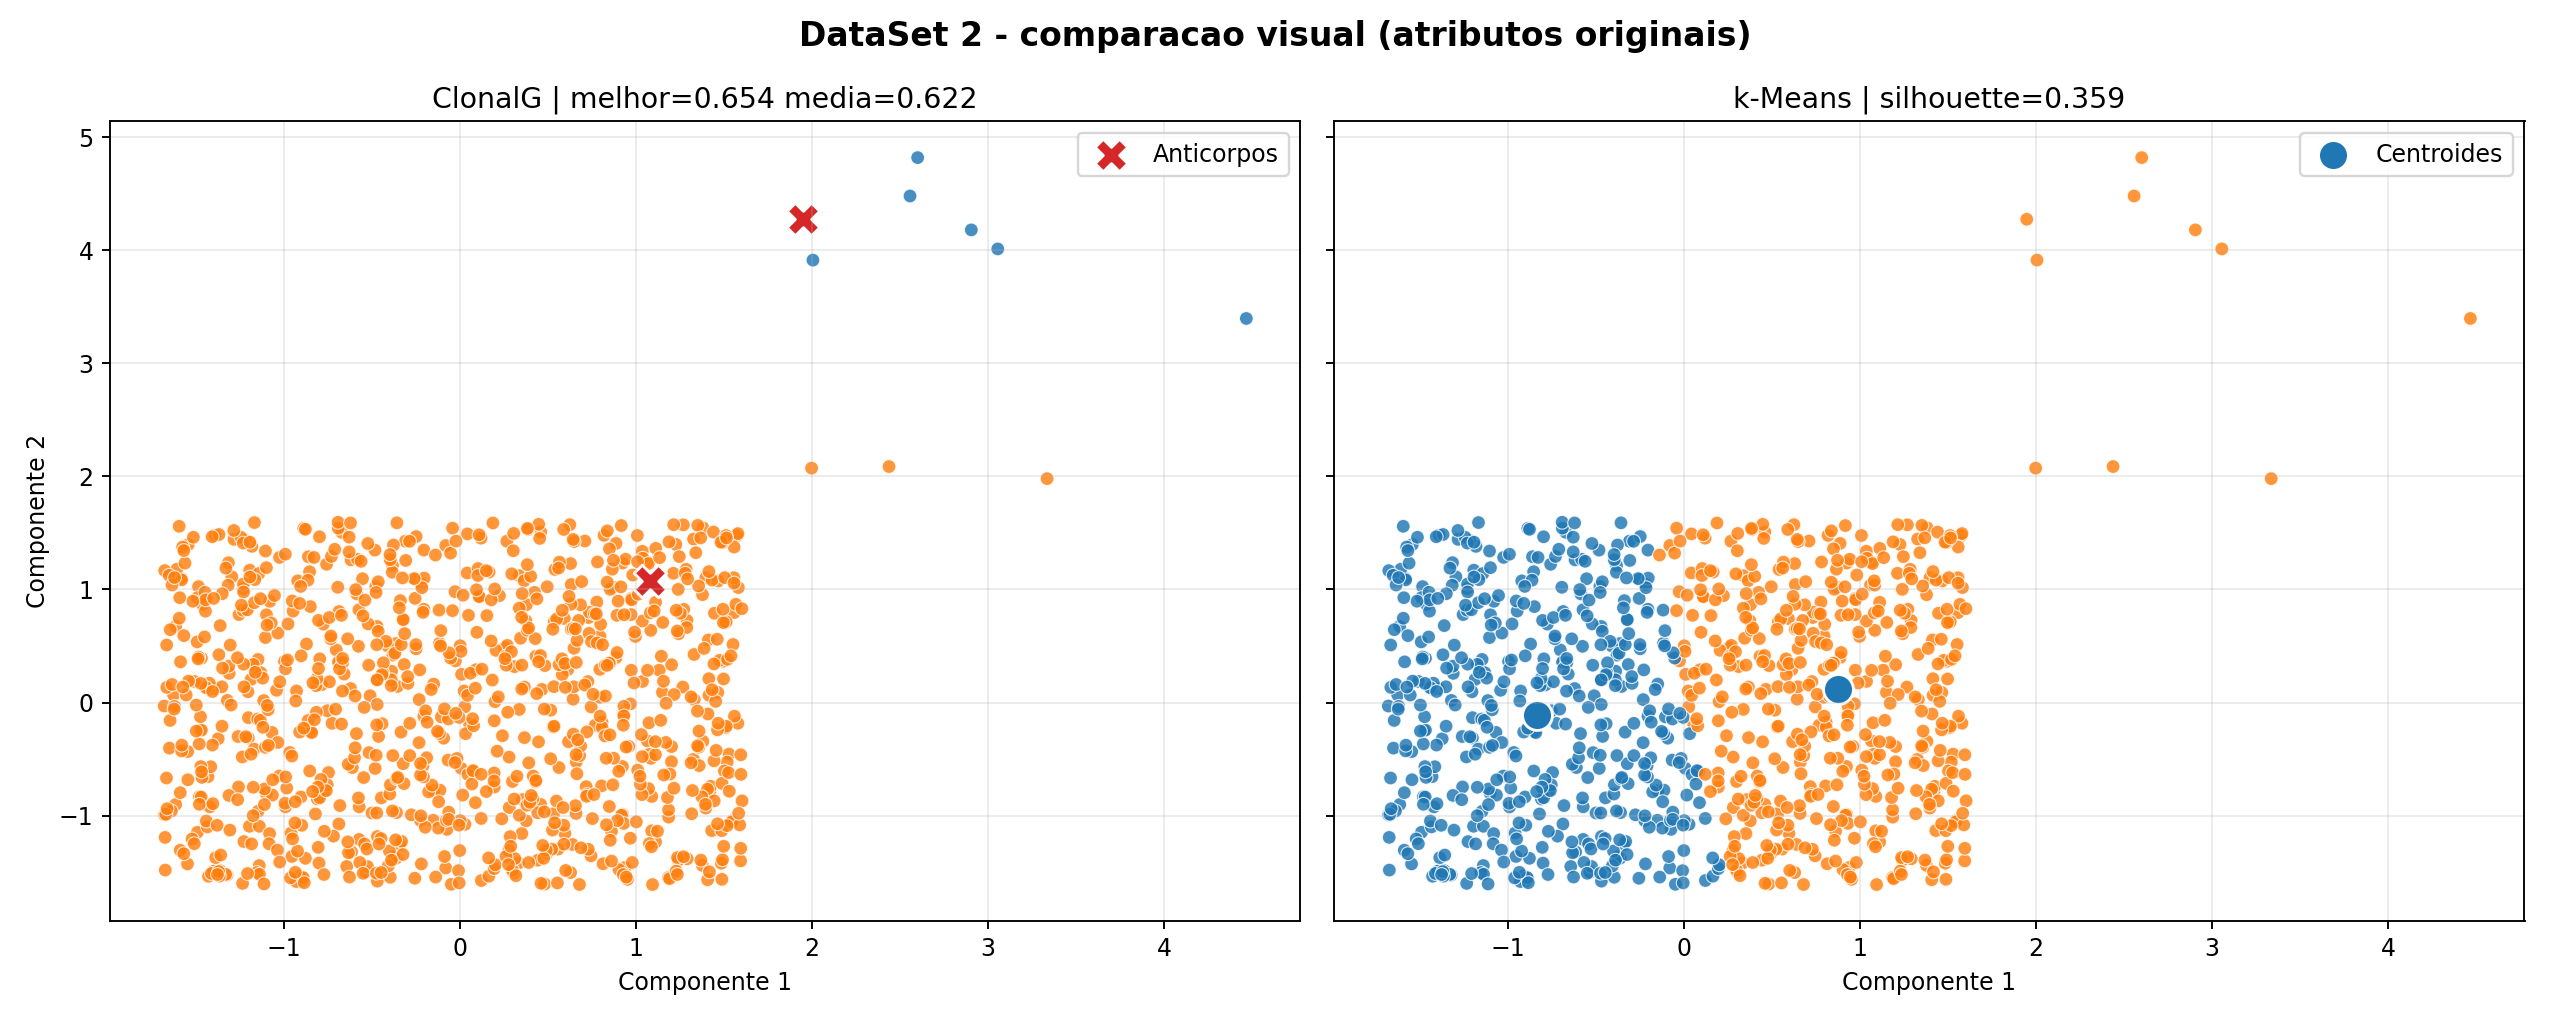
\includegraphics[width=\textwidth]{resultados/comparativo_final/comparacao_ds2.png}
      \end{center}
    \end{column}
    \begin{column}{0.38\textwidth}
      \textbf{Análise do DataSet 2:}
      \begin{itemize}
        \item \textbf{k-Means (Direita):} Fica preso em um mínimo local artificial, fundindo grupos reais.
        \item \textbf{ClonalG Otimizado (Esquerda):} Separação nítida em dois clusters coerentes.
        \item A combinação de mutação paramétrica contínua e diversidade populacional evitou a convergência prematura.
      \end{itemize}
    \end{column}
  \end{columns}
\end{frame}

\begin{frame}{Resultados de Convergência}{Curva de Evolução no DataSet 2}
  \begin{columns}
    \begin{column}{0.48\textwidth}
      \begin{center}
        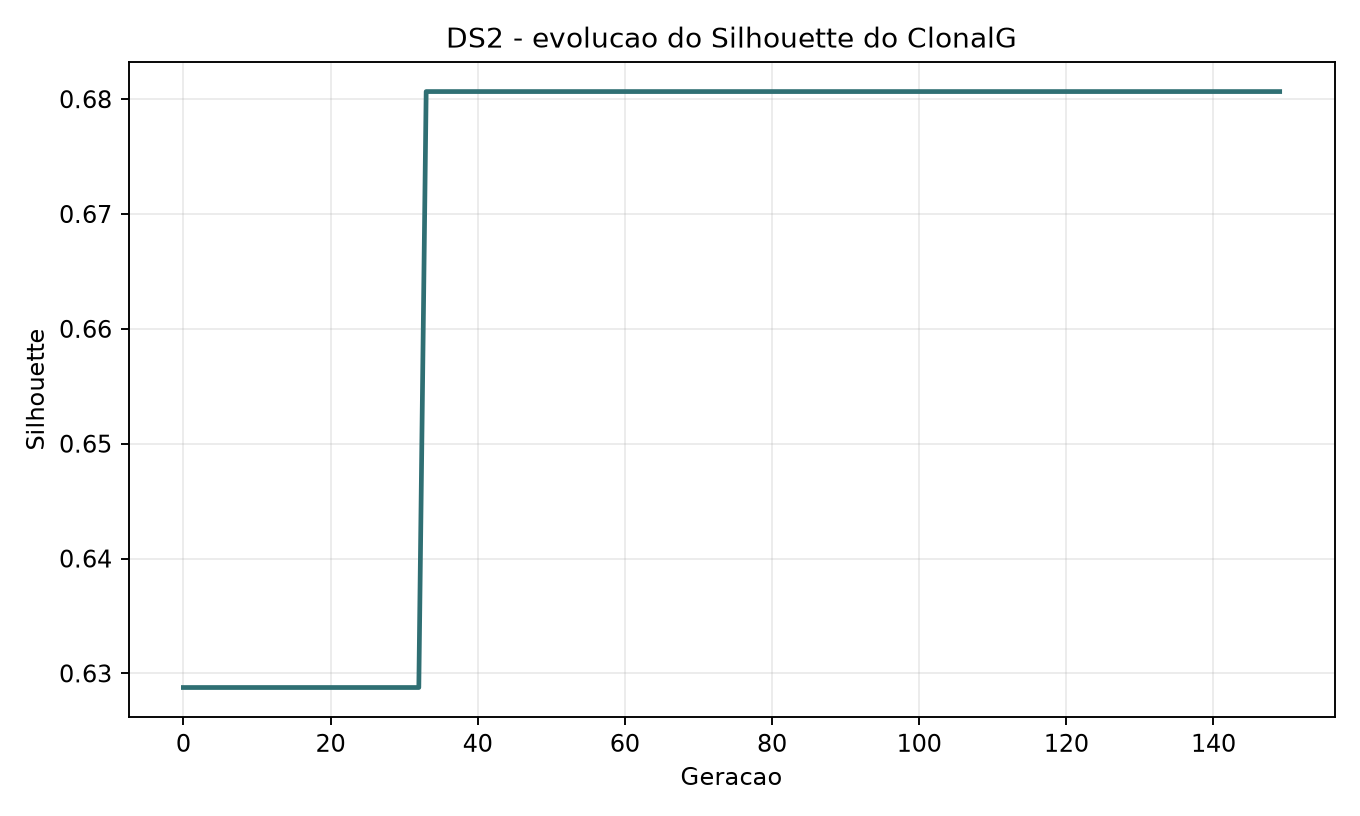
\includegraphics[width=0.95\textwidth]{resultados/comparativo_final/evolucao_clonalg_ds2.png}
      \end{center}
    \end{column}
    \begin{column}{0.52\textwidth}
      \textbf{Comportamento da Evolução:}
      \begin{itemize}
        \item A afinidade (Índice Silhouette) cresce rapidamente nas primeiras 10 gerações.
        \item A mutação paramétrica contínua age refinando localmente as soluções.
        \item A estabilização ocorre de maneira suave, indicando robustez e convergência estável do sistema.
      \end{itemize}
    \end{column}
  \end{columns}
\end{frame}

\begin{frame}{Discussão dos Resultados}
  \begin{itemize}
    \item \textbf{Superação do k-Means no DS2:}
      \begin{itemize}
        \item O k-Means ficou preso em mínimos locais devido à inicialização. O ClonalG, graças à busca estocástica global e à mutação paramétrica contínua, localizou a separação ótima estável.
      \end{itemize}
    \item \textbf{Impacto da Diversidade:}
      \begin{itemize}
        \item A seleção de memória guiada por diversidade manteve múltiplos candidatos ativos, permitindo encontrar o número correto de clusters mesmo sob geometrias complexas.
      \end{itemize}
    \item \textbf{Busca Contínua vs. Discreta:}
      \begin{itemize}
        \item A busca paramétrica refinou as coordenadas reais dos centroides, gerando limites de decisão mais suaves e aumentando a métrica do Silhouette.
      \end{itemize}
  \end{itemize}
\end{frame}

\begin{frame}{Conclusões}
  \begin{itemize}
    \item O algoritmo ClonalG melhorado provou ser uma alternativa robusta e adaptativa ao clássico k-Means.
    \item As melhorias propostas (busca local contínua via ruído gaussiano adaptativo e nichamento por diversidade) sanaram a convergência prematura típica do SIA básico.
    \item \textbf{Trabalhos Futuros:} Testar outras métricas de afinidade além do Silhouette (como Davies-Bouldin) e automatizar o decaimento dinâmico dos hiperparâmetros de mutação ao longo das gerações.
  \end{itemize}
\end{frame}

\end{document}
